\let\negmedspace\undefined
\let\negthickspace\undefined
\documentclass[journal]{IEEEtran}
\usepackage[a5paper, margin=10mm, onecolumn]{geometry}
%\usepackage{lmodern} % Ensure lmodern is loaded for pdflatex
\usepackage{tfrupee} % Include tfrupee package

\setlength{\headheight}{1cm} % Set the height of the header box
\setlength{\headsep}{0mm}     % Set the distance between the header box and the top of the text

\usepackage{gvv-book}
\usepackage{gvv}
\usepackage{cite}
\usepackage{amsmath,amssymb,amsfonts,amsthm}
\usepackage{algorithmic}
\usepackage{graphicx}
\usepackage{textcomp}
\usepackage{xcolor}
\usepackage{txfonts}
\usepackage{listings}
\usepackage{enumitem}
\usepackage{mathtools}
\usepackage{gensymb}
\usepackage{comment}
\usepackage[breaklinks=true]{hyperref}
\usepackage{tkz-euclide} 
\usepackage{listings}
% \usepackage{gvv}                                        
\def\inputGnumericTable{}                                 
\usepackage[latin1]{inputenc}                                
\usepackage{color}                                            
\usepackage{array}                                            
\usepackage{longtable}                                       
\usepackage{calc}                                             
\usepackage{multirow}                                         
\usepackage{hhline}                                           
\usepackage{ifthen}                                           
\usepackage{lscape}
\begin{document}

\bibliographystyle{IEEEtran}
\vspace{3cm}

\title{4.7.57}
\author{EE25BTECH11060 - V.Namaswi}
% \maketitle
% \newpage
% \bigskip
{\let\newpage\relax\maketitle}

\renewcommand{\thefigure}{\theenumi}
\renewcommand{\thetable}{\theenumi}
\setlength{\intextsep}{10pt} % Space between text and floats
\textbf{Question}\\  
Find distance of $\brak{3,-5}$ from line 3x-4y-26=0\\
 \textbf{Solution:}\\
The given line is
\[
3x - 4y - 26 = 0
\]
This can be written in the form 
\begin{align}
\Vec{n}^\top \Vec{x}= c
\end{align}
where 
\[
\Vec{n}= \begin{pmatrix} 3 \\ -4 \end{pmatrix}, 
\quad c = 26.
\]

Let the point be 
\[
\Vec{P} = \begin{pmatrix} 3 \\ -5 \end{pmatrix}.
\]

The distance of point \(\Vec{P}\) from the line is
\begin{align}
d = \frac{|\Vec{n}^\top \Vec{P} - c|}{\|\Vec{n}\|}.
\end{align}

Substituting the values,
\begin{align}
\Vec{n}^\top \Vec{P} = \begin{pmatrix} 3 & -4 \end{pmatrix}
\begin{pmatrix} 3 \\ -5 \end{pmatrix}\\
= 3(3) + (-4)(-5)\\ = 9 + 20 = 29.\\
\Vec{n}^\top \vec{P} - c\\ = 29 - 26 = 3.\\
\|\vec{n}\| = \sqrt{3^2 + (-4)^2}\\ = \sqrt{9+16} = 5.\\
So,
d = \frac{|3|}{5} = \frac{3}{5}.
\end{align}
Refer fig
 \centering
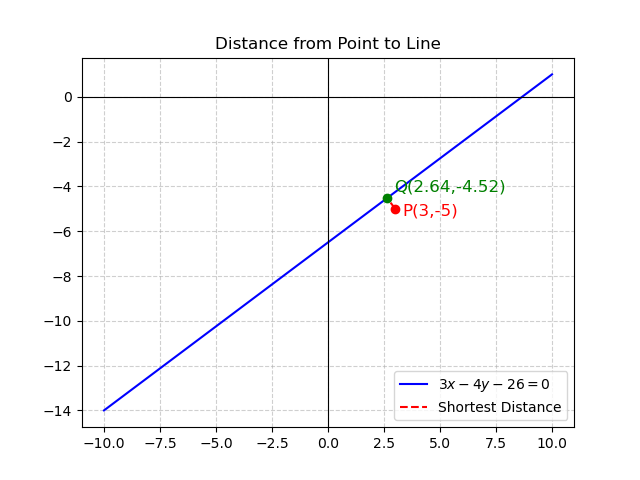
\includegraphics[width=\columnwidth, height=0.8\textheight, keepaspectratio]{figs/Figure_7.png}     
\end{document}